\section{可重构计算}

\subsection{英文论文}

搜索关键词问可重构计算的英文论文的过程为,在IEEE xplore的ADVANCED SEARCH中输入reconfigurable computing,然后点击搜索。

\begin{figure}[H]
    \centering
    \begin{subfigure}{0.8\textwidth}
        \centering
        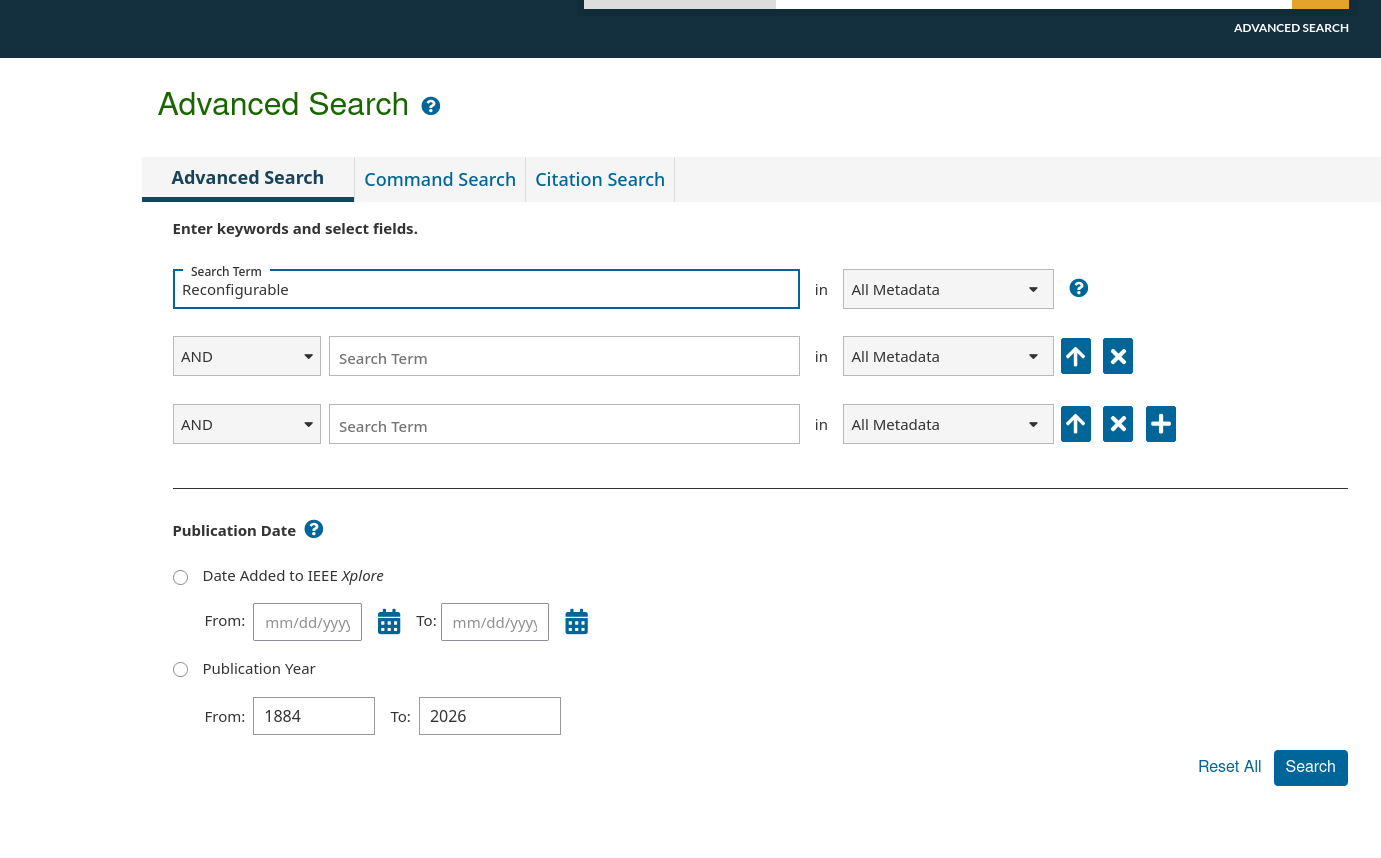
\includegraphics[width=0.7\textwidth]{./asserts/reconfigurable_computing_search.png}
        \caption{Advanced search}
    \end{subfigure}

    % \hfill

    \begin{subfigure}{0.8\textwidth}
        \centering
        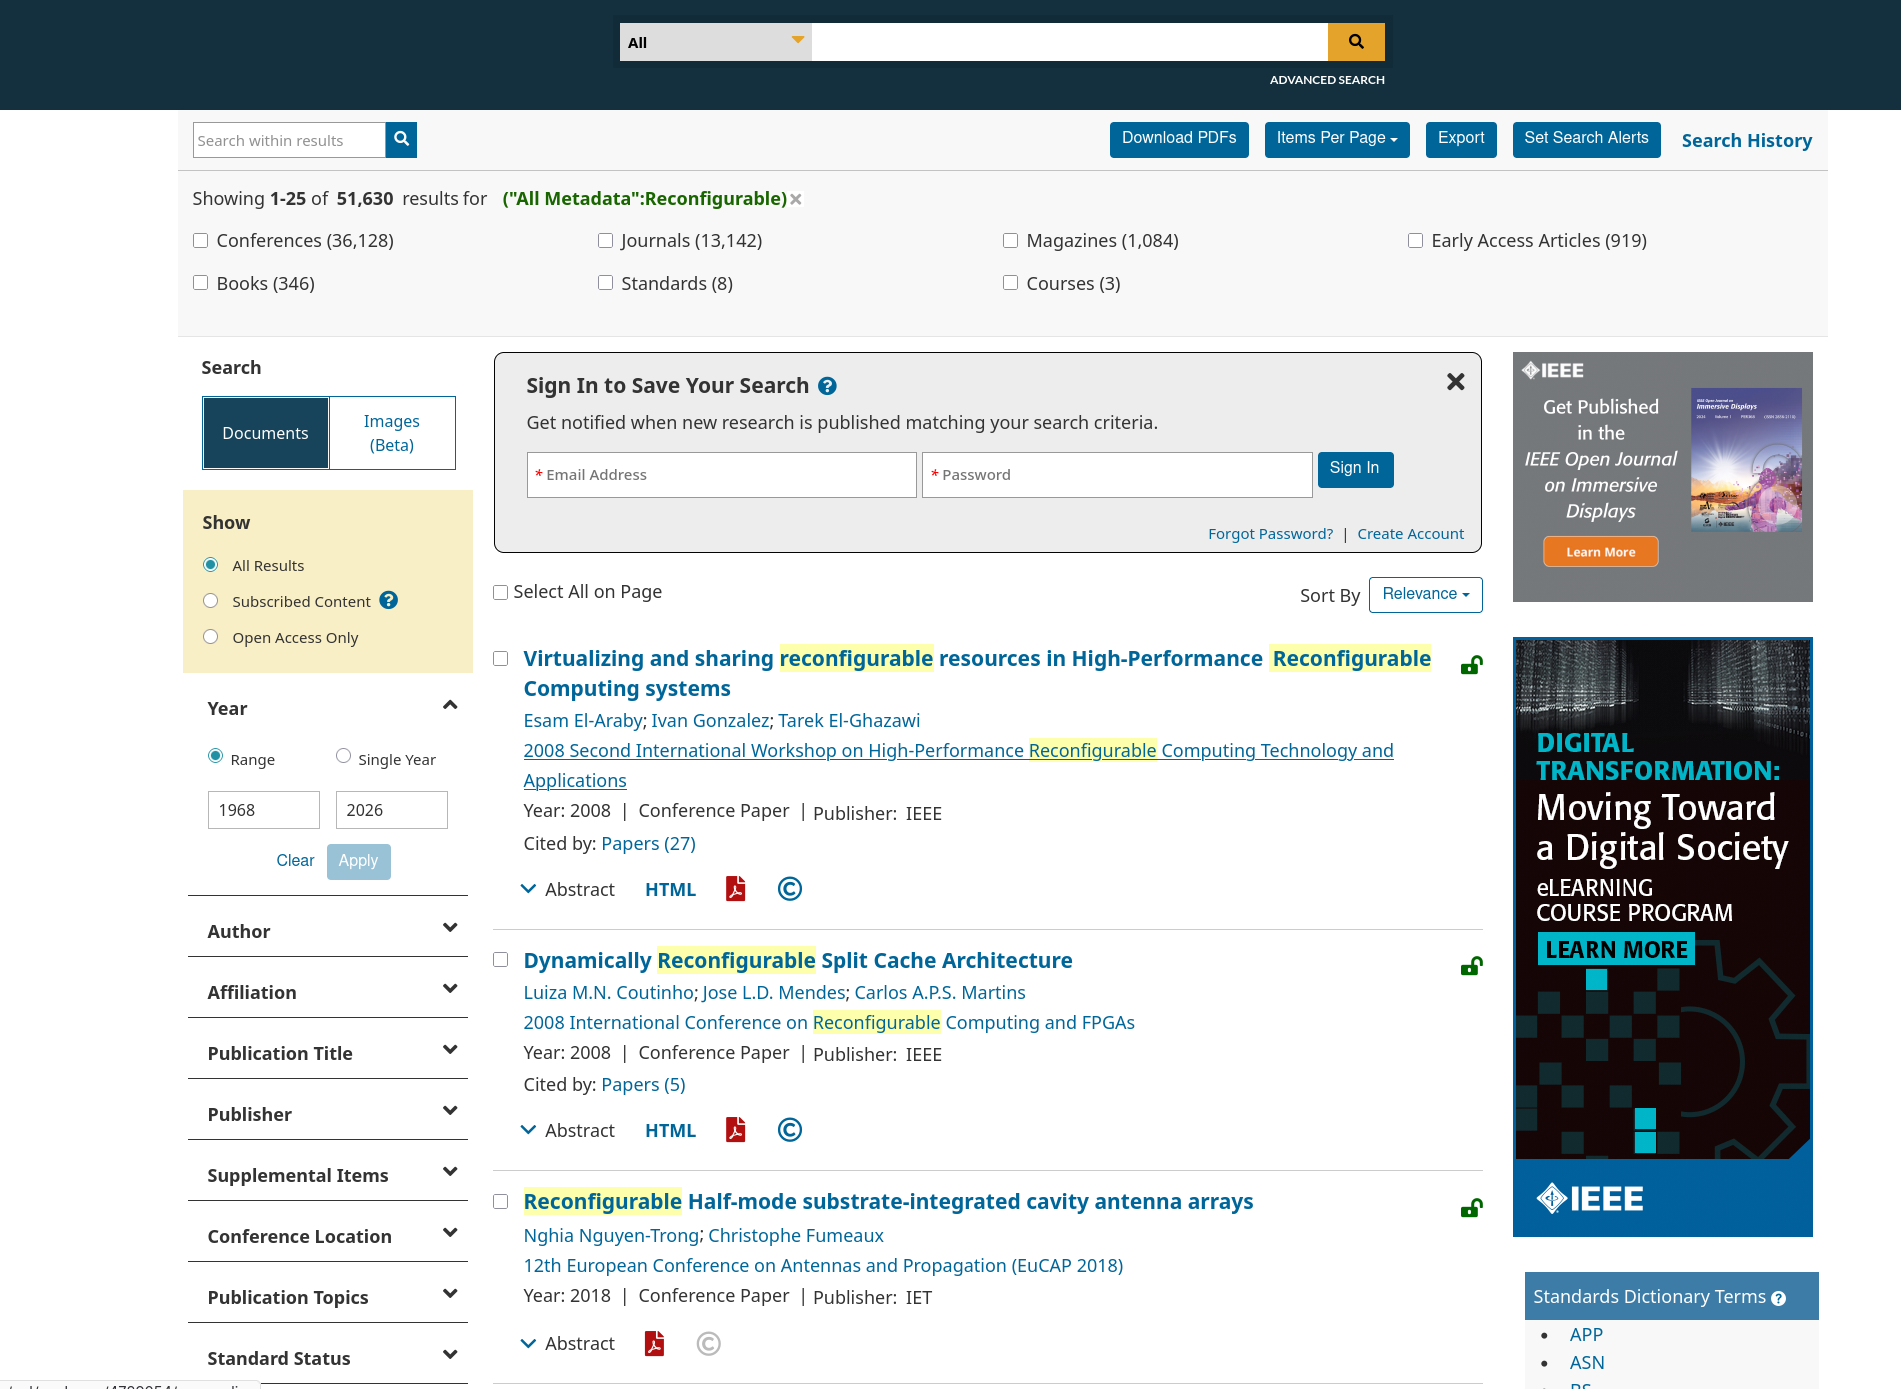
\includegraphics[width=0.7\textwidth]{./asserts/reconfg_res_en.png}
        \caption{Search result}
    \end{subfigure}
\end{figure}


\begin{itemize}
    % 论文题目
    \item 论文名:Resource Awareness FPGA Design Practices for Reconfigurable Computing: Principles and Examples

    % 作者信息
    \item 作者信息:
        \begin{enumerate}
            \item Jinyuan Wu:
                \begin{itemize}
                    \item Fenni National Accelerator Laboratory, Batavia, IL, USA
                \end{itemize}
        \end{enumerate}

    % 收录信息(会议 / 期刊)
    \item 收录情况:
        \begin{itemize}
            \item Published in: 2007 15th IEEE-NPSS Real-Time Conference
            \item DOI: 10.1109/RTC.2007.4382752
        \end{itemize}

    % 影响因子(若是会议则标明“无影响因子”)
    \item 影响因子:会议论文无影响因子

    % 引用情况(如果有后续引用)
    \item 被引情况:
        \begin{itemize}
            \item N. M. Salgado-Herrera, Aurelio Medina-Ríos, Antonio Ramos-Paz, J. R. Rodríguez-Rodríguez, "Generation of a multilevel SPWM technique of 3, 9 and 21 levels with FPGAs", 2013 North American Power Symposium (NAPS), pp.1-5, 2013.
            % 可继续添加引用
        \end{itemize}
\end{itemize}

% This is template
% \begin{itemize}
%     % 论文题目
%     \item 论文名:<Title in English or 中文>
% 
%     % 作者信息
%     \item 作者信息:
%         \begin{enumerate}
%             \item <Author1>:
%                 \begin{itemize}
%                     \item <Affiliation 1>
%                     \item <Affiliation 2 (若有)>
%                 \end{itemize}
%             \item <Author2>:
%                 \begin{itemize}
%                     \item <Affiliation 1>
%                 \end{itemize}
%             % ……按需添加更多作者
%         \end{enumerate}
% 
%     % 收录信息(会议 / 期刊)
%     \item 收录情况:
%         \begin{itemize}
%             \item Published in: <Conference / Journal Name> (<Year>)
%             \item DOI: <DOI Number>
%         \end{itemize}
% 
%     % 影响因子(若是会议则标明“无影响因子”)
%     \item 影响因子:<期刊 IF / 会议论文无影响因子>
% 
%     % 引用情况(如果有后续引用)
%     \item 被引情况:
%         \begin{itemize}
%             \item <Author list>, "<Title>", <Conference/Journal>, pp.xx--xx, <Year>.
%             % 可继续添加引用
%         \end{itemize}
% \end{itemize}


\subsection{中文论文}
